\chapter{Экспериментальный раздел}
\label{cha:research}

В рамках дипломного проекта был проведен ряд экспериментов, направленных на исследование метода выделения голосовой составляющей из монофонического аудио сигнала. 

В качестве входных данных использовались музыкальные композиции с мужским и женским вокалом. Так же аккомпанимент мог быть записан либо с использованием музыкальных инструментов, либо при помощи цифровой звуковой рабочей станции.

\section{Описание используемой модели}

Обучение модели было произведено один раз за 150 эпох. Данный процесс занял 20 дней. Для обучения использовалась обучающая часть набора данных DSD100. График изменения ошибки в процессе обучения представлен на рисунке \ref{res:loss}.

\begin{figure}
	\centering
	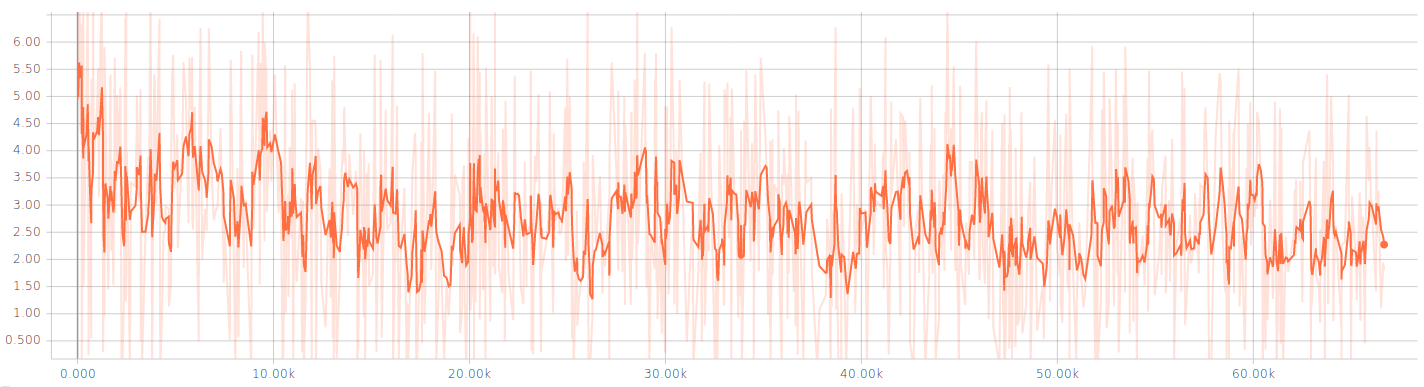
\includegraphics[width=\textwidth]{inc/img/loss-dsd}
	\caption{График изменения ошибки}
	\label{res:loss}
\end{figure}

\section{Описание тестирующей выборки}

Набор данных DSD100 состоит как из данных для обучения нейронной сети, так и из данных для ее проверки.  Данные из этого набора были приведены к двухканальному wav-файлу со следующей структурой:

\begin{itemize}
	\item Левый канал -- аккомпанимент.
	\item Правый канал -- голосовая составляющая.
\end{itemize}

\section{Методика проведения исследования}

Проведение эксперимента происходило на всей тестовой выборке набора данных DSD100. Каждый аудио файл проходил обработку разработанным методом и для полученных аудио сигналов голосовой составляющей и аккомпанемента вычислялись метрики SDR, SIR, SAR и ISR, описанные выше.

Среди полученных метрик находились максимальные и минимальные значения. На основании этих чисел определялись средние значения метрик и их разброс.

Сравнение полученных результатов с результатами методов, описанных ранее, представлено в таблице \ref{res:canonsummary}.

\begin{table}[h]
	\caption{\label{res:canonsummary}Сравнение алгоритмов выделения источников}
	\begin{center}
		\begin{tabular}{|c|c|c|c|}
			\hline
			Метод & Метрика & Вокал & Аккомпанемент \\
			\hline
			РНС & SDR & -0.6 ± 4.9 & 4.5 ± 1.2 \\
			& SIR & 1.9 ± 6.2 & 14.9 ± 5.6 \\
			& SAR & 3.6 ± 2.1 & 16.4 ± 2.9 \\
			& ISR & 7.3 ± 2.7 & 6.9 ± 1.0 \\
			\hline
			ГНС & SDR & -8.9 ± 4.4 & 4.1 ± 2.6 \\
			& SIR & 10.8 ± 3.1 & 10.7 ± 3.8 \\
			& SAR & -6.6 ± 4.6 & 12.1 ± 3.9 \\
			& ISR & 4.8 ± 2.8 & 5.0 ± 3.0 \\
			\hline
			FASST & SDR & -1.8 ± 5.8 & 8.9 ± 3.2 \\
			& SIR & -3.7 ± 7.5 & 13.7 ± 3.0 \\
			& SAR & 4.3 ± 1.4 & 13.1 ± 3.2 \\
			& ISR & 5.6 ± 2.5 & 13.5 ± 2.5 \\
			\hline
			\textbf{Глубинные РНС} & SDR & -5.6 ± 1.2 & 7.3 ± 4.2 \\
			& SIR & -3.6 ± 2.5 & 10.5 ± 1.8 \\
			& SAR & 3.8 ± 1.4 & 10.4 ± 3.2 \\
			& ISR & 5.3 ± 2.5 & 5.1 ± 2.5 \\
			\hline
		\end{tabular}
	\end{center}
\end{table} 

\section{Спектрограммы}

Были проведены сравнения спектрограмм полученных аудио сигналов с ожидаемыми. Сравнения проводились для двух музыкальных произведений: с мужским вокалом и женским вокалом.

Спектрограммы сигналов голосовой составляющей и аккомпанемента музыкального произведения с мужским вокалом представлены на рисунках \ref{res:malevoice} и  \ref{res:malemusic} соответственно.

Спектрограммы сигналов голосовой составляющей и аккомпанемента музыкального произведения с женским вокалом представлены на рисунках \ref{res:femalevoice} и  \ref{res:femalemusic} соответственно.

\begin{figure}
	\centering
	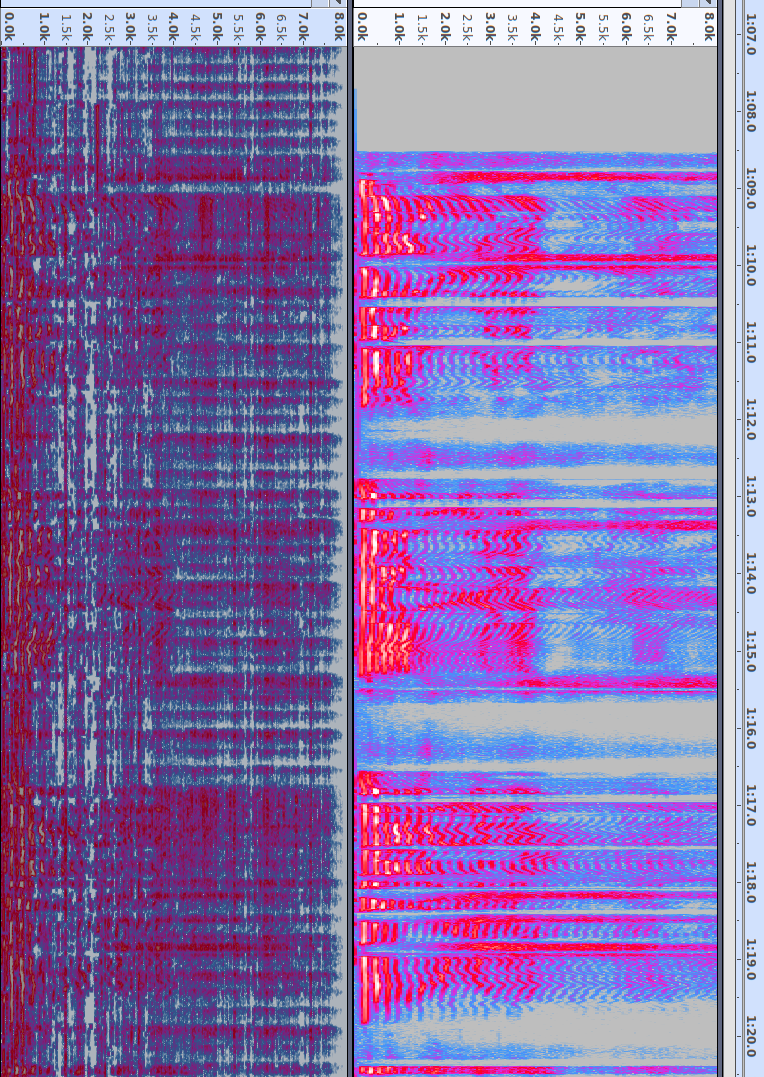
\includegraphics[width=0.9\textwidth]{inc/img/spec-voice-male}
	\caption{Сравнение спектрограмм голосовых составляющих музыкального произведения с мужским вокалом. Сверху: спектрограмма ожидаемого сигнала, снизу: спектрограмма полученного сигнала}
	\label{res:malevoice}
\end{figure}

\begin{figure}
	\centering
	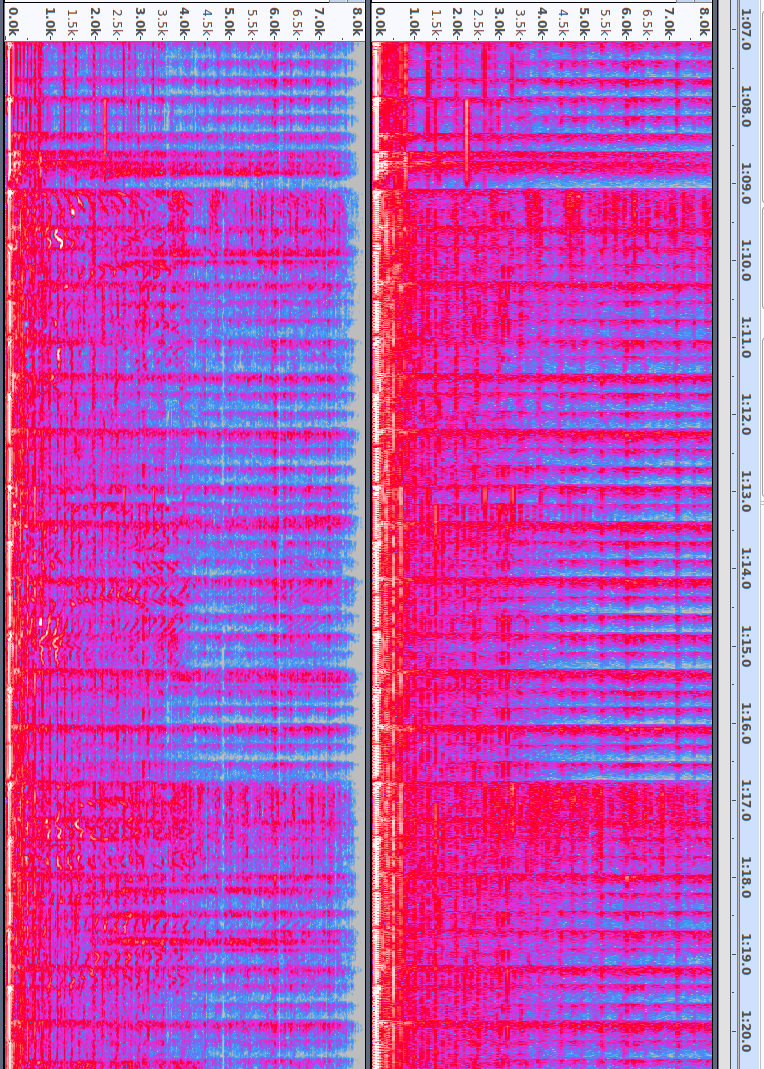
\includegraphics[width=0.9\linewidth]{inc/img/spec-music-male}
	\caption{Сравнение спектрограмм аккомпанемента музыкального произведения с мужским вокалом. Сверху: спектрограмма ожидаемого сигнала, снизу: спектрограмма полученного сигнала}
	\label{res:malemusic}
\end{figure}

\begin{figure}
	\centering
	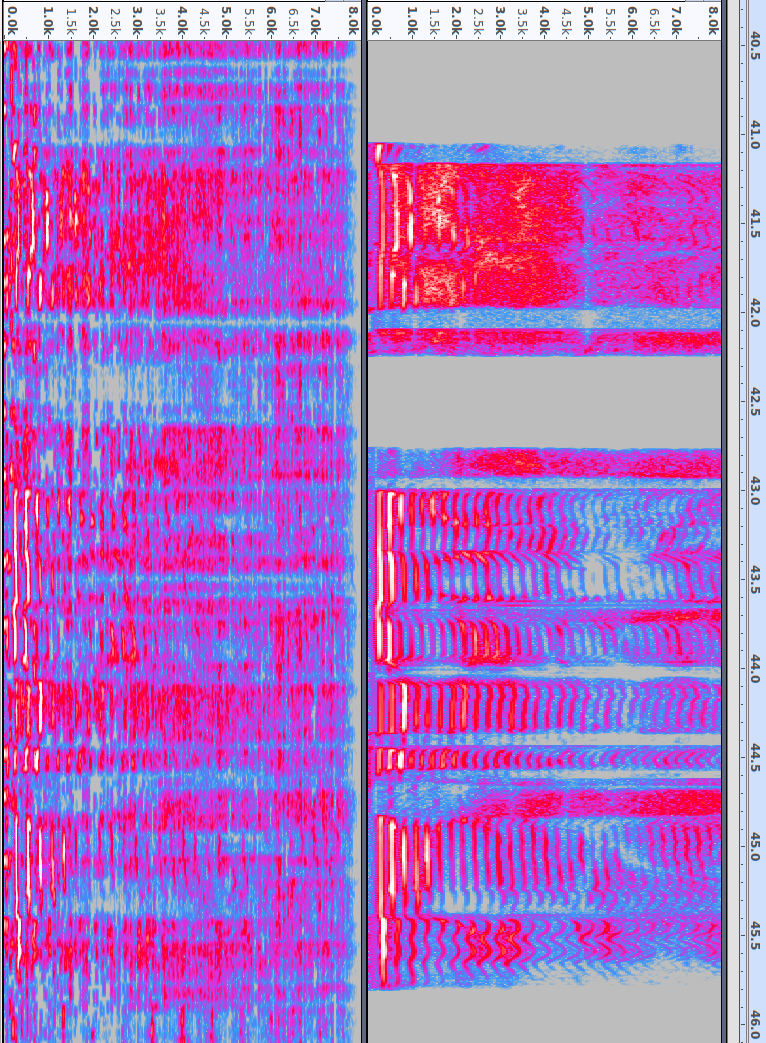
\includegraphics[width=0.9\textwidth]{inc/img/spec-voice-female}
	\caption{Сравнение спектрограмм голосовых составляющих музыкального произведения с женским вокалом. Сверху: спектрограмма ожидаемого сигнала, снизу: спектрограмма полученного сигнала}
	\label{res:femalevoice}
\end{figure}

\begin{figure}
	\centering
	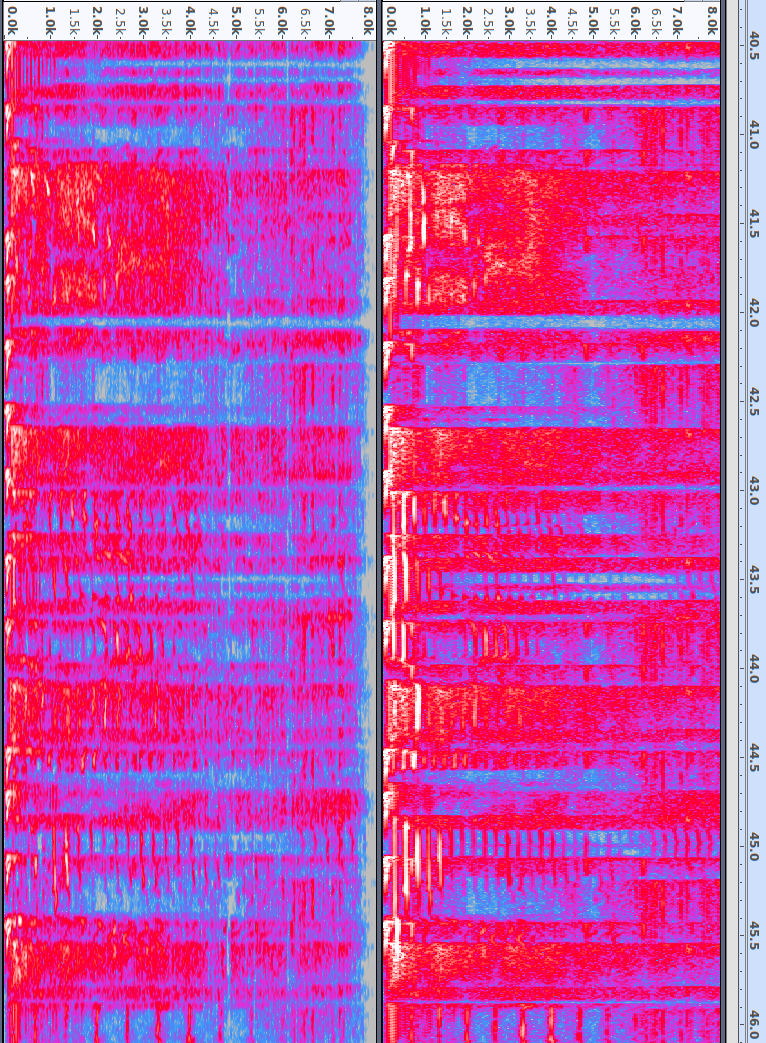
\includegraphics[width=0.9\textwidth]{inc/img/spec-music-female}
	\caption{Сравнение спектрограмм аккомпанемента музыкального произведения с женским вокалом. Сверху: спектрограмма ожидаемого сигнала, снизу: спектрограмма полученного сигнала}
	\label{res:femalemusic}
\end{figure}


%%% Local Variables:
%%% mode: latex
%%% TeX-master: "rpz"
%%% End:
